

\tikzset{every picture/.style={line width=0.75pt}} %set default line width to 0.75pt        

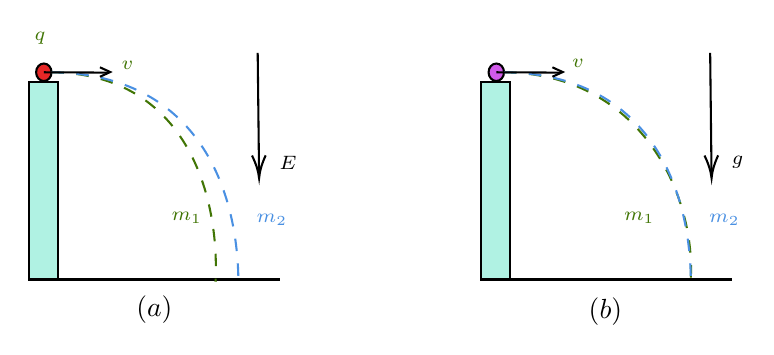
\begin{tikzpicture}[x=0.75pt,y=0.75pt,yscale=-1,xscale=1]
%uncomment if require: \path (0,208); %set diagram left start at 0, and has height of 208

%Straight Lines [id:da7700030123349858] 
\draw    (135.68,158.23) -- (256.68,158.23) ;
%Shape: Rectangle [id:dp29978224875973536] 
\draw  [fill={rgb, 255:red, 80; green, 227; blue, 194 }  ,fill opacity=0.45 ] (135.68,63.25) -- (149.68,63.25) -- (149.68,158.23) -- (135.68,158.23) -- cycle ;
%Shape: Ellipse [id:dp8627118519329677] 
\draw  [fill={rgb, 255:red, 226; green, 3; blue, 3 }  ,fill opacity=0.86 ] (139.24,58.39) .. controls (139.24,56.06) and (140.9,54.17) .. (142.96,54.17) .. controls (145.02,54.17) and (146.68,56.06) .. (146.68,58.39) .. controls (146.68,60.71) and (145.02,62.6) .. (142.96,62.6) .. controls (140.9,62.6) and (139.24,60.71) .. (139.24,58.39) -- cycle ;
%Curve Lines [id:da7221212930215757] 
\draw [color={rgb, 255:red, 65; green, 117; blue, 5 }  ,draw opacity=1 ] [dash pattern={on 4.5pt off 4.5pt}]  (146.68,58.39) .. controls (212.68,59.02) and (227.68,119.3) .. (225.68,159.3) ;
%Curve Lines [id:da9277583988258424] 
\draw [color={rgb, 255:red, 74; green, 144; blue, 226 }  ,draw opacity=1 ] [dash pattern={on 4.5pt off 4.5pt}]  (146.68,58.39) .. controls (212.68,59.02) and (235.68,108.3) .. (236.68,157.3) ;
%Straight Lines [id:da669874321545674] 
\draw    (246,49) -- (246.66,107.4) ;
\draw [shift={(246.68,109.4)}, rotate = 269.35] [color={rgb, 255:red, 0; green, 0; blue, 0 }  ][line width=0.75]    (10.93,-3.29) .. controls (6.95,-1.4) and (3.31,-0.3) .. (0,0) .. controls (3.31,0.3) and (6.95,1.4) .. (10.93,3.29)   ;
%Straight Lines [id:da7821967004831883] 
\draw    (353.68,158.23) -- (474.68,158.23) ;
%Shape: Rectangle [id:dp4966288179818329] 
\draw  [fill={rgb, 255:red, 80; green, 227; blue, 194 }  ,fill opacity=0.45 ] (353.68,63.25) -- (367.68,63.25) -- (367.68,158.23) -- (353.68,158.23) -- cycle ;
%Shape: Ellipse [id:dp2216871915879428] 
\draw  [fill={rgb, 255:red, 189; green, 16; blue, 224 }  ,fill opacity=0.69 ] (357.24,58.39) .. controls (357.24,56.06) and (358.9,54.17) .. (360.96,54.17) .. controls (363.02,54.17) and (364.68,56.06) .. (364.68,58.39) .. controls (364.68,60.71) and (363.02,62.6) .. (360.96,62.6) .. controls (358.9,62.6) and (357.24,60.71) .. (357.24,58.39) -- cycle ;
%Curve Lines [id:da19048860688087488] 
\draw [color={rgb, 255:red, 65; green, 117; blue, 5 }  ,draw opacity=1 ] [dash pattern={on 4.5pt off 4.5pt}]  (364.68,58.39) .. controls (430.68,59.02) and (456.68,117.3) .. (454.68,157.3) ;
%Curve Lines [id:da9137169483322104] 
\draw [color={rgb, 255:red, 74; green, 144; blue, 226 }  ,draw opacity=1 ] [dash pattern={on 4.5pt off 4.5pt}]  (364.68,58.39) .. controls (430.68,59.02) and (453.68,108.3) .. (454.68,157.3) ;
%Straight Lines [id:da4783383221798906] 
\draw    (464,49) -- (464.66,107.4) ;
\draw [shift={(464.68,109.4)}, rotate = 269.35] [color={rgb, 255:red, 0; green, 0; blue, 0 }  ][line width=0.75]    (10.93,-3.29) .. controls (6.95,-1.4) and (3.31,-0.3) .. (0,0) .. controls (3.31,0.3) and (6.95,1.4) .. (10.93,3.29)   ;
%Straight Lines [id:da750649433001236] 
\draw    (142.96,58.39) -- (173.96,58.55) ;
\draw   (170,56) -- (174.96,58.27) -- (170,60.55) ;
%Straight Lines [id:da025640929368151655] 
\draw    (360.96,58.39) -- (391.96,58.55) ;
\draw   (388,56) -- (392.96,58.27) -- (388,60.55) ;


% Text Node
\draw (203,124.4) node [anchor=north west][inner sep=0.75pt]  [font=\scriptsize,color={rgb, 255:red, 65; green, 117; blue, 5 }  ,opacity=1 ]  {$m_{1}$};
% Text Node
\draw (244,125.4) node [anchor=north west][inner sep=0.75pt]  [font=\scriptsize,color={rgb, 255:red, 74; green, 144; blue, 226 }  ,opacity=1 ]  {$m_{2}$};
% Text Node
\draw (137,37.4) node [anchor=north west][inner sep=0.75pt]  [font=\scriptsize,color={rgb, 255:red, 65; green, 117; blue, 5 }  ,opacity=1 ]  {$q\ $};
% Text Node
\draw (255,97.4) node [anchor=north west][inner sep=0.75pt]  [font=\scriptsize]  {$\vb{E}$};
% Text Node
\draw (421,124.4) node [anchor=north west][inner sep=0.75pt]  [font=\scriptsize,color={rgb, 255:red, 65; green, 117; blue, 5 }  ,opacity=1 ]  {$m_{1}$};
% Text Node
\draw (462,125.4) node [anchor=north west][inner sep=0.75pt]  [font=\scriptsize,color={rgb, 255:red, 74; green, 144; blue, 226 }  ,opacity=1 ]  {$m_{2}$};
% Text Node
\draw (396,50.4) node [anchor=north west][inner sep=0.75pt]  [font=\scriptsize,color={rgb, 255:red, 65; green, 117; blue, 5 }  ,opacity=1 ]  {$\vb{v}$};
% Text Node
\draw (473,97.4) node [anchor=north west][inner sep=0.75pt]  [font=\scriptsize]  {$\vb{g}$};
% Text Node
\draw (186,164.4) node [anchor=north west][inner sep=0.75pt]    {$( a)$};
% Text Node
\draw (404,165.4) node [anchor=north west][inner sep=0.75pt]    {$( b)$};
% Text Node
\draw (179,51.4) node [anchor=north west][inner sep=0.75pt]  [font=\scriptsize,color={rgb, 255:red, 65; green, 117; blue, 5 }  ,opacity=1 ]  {$\vb{v}\ $};


\end{tikzpicture}
